\documentclass[a4paper,fleqn]{cas-dc}

\usepackage{amsmath,amssymb}
\usepackage{booktabs}
\usepackage{array}
\usepackage{graphicx}
\usepackage[numbers,sort&compress]{natbib}
\usepackage{microtype}
\usepackage{url}
\usepackage{enumitem}
\usepackage{placeins}
\usepackage{adjustbox}
\usepackage{silence}
\WarningFilter{hyperref}{Ignoring empty anchor}
\IfFileExists{CharisSIL.sty}{\usepackage{CharisSIL}}{\microtypesetup{expansion=false}}

\emergencystretch=3em
\hbadness=10000
\setlength{\textfloatsep}{9pt plus 2pt minus 2pt}
\setlength{\floatsep}{7pt plus 2pt minus 2pt}
\setlength{\intextsep}{8pt plus 2pt minus 2pt}
\setlength{\dbltextfloatsep}{9pt plus 2pt minus 2pt}
\setlength{\dblfloatsep}{7pt plus 2pt minus 2pt}
\renewcommand{\topfraction}{0.95}
\renewcommand{\bottomfraction}{0.85}
\renewcommand{\textfraction}{0.05}
\renewcommand{\floatpagefraction}{0.85}
\renewcommand{\dbltopfraction}{0.95}
\renewcommand{\dblfloatpagefraction}{0.85}
\pdfstringdefDisableCommands{\def\corref#1{}}

\graphicspath{{figures/}}
\newcommand{\AP}{\mathrm{AP}}
\newcommand{\appts}{\,\text{AP points}}
\newcolumntype{Y}[1]{>{\raggedright\arraybackslash}p{#1}}

\begin{document}
\begin{titlepage}
\shortauthors{Nguyen et al.}
\shorttitle{Paired, floor-guarded INT8--FP8 evaluation}
\title[mode=title]{A Paired, Floor-Guarded Evaluation Protocol for TensorRT INT8 and FP8 Object Detectors under Synthetic Image Corruptions}

\author[mymainaddress]{Dinh Thuan Nguyen}[orcid=0000-0001-9302-3129]
\author[mymainaddress]{Lam Phuong Nguyen}[orcid=0009-0007-3439-5871]
\author[mysecondaryaddress]{Vinh Huy Nguyen}[orcid=0009-0006-0878-9714]
\author[mythirdaddress]{Mohan Rajesh Elara}[orcid=0000-0001-6504-1530]
\author[myfourthaddress]{Anh Vu Le\corref{mycorrespondingauthor}}[orcid=0000-0002-4804-7540]
\cortext[mycorrespondingauthor]{Corresponding author: \href{mailto:leanhvu@tdtu.edu.vn}{leanhvu@tdtu.edu.vn}.}

\address[mymainaddress]{Faculty of Electrical and Electronics Engineering, Ton Duc Thang University, Ho Chi Minh City, Vietnam}
\address[mysecondaryaddress]{Center of Visualization and Simulation, Duy Tan University, Da Nang, Vietnam}
\address[mythirdaddress]{ROAR Lab, Engineering Product Development, Singapore University of Technology and Design, Singapore}
\address[myfourthaddress]{Advanced Intelligent Technology Research Group, Faculty of Electrical and Electronics Engineering, Ton Duc Thang University, Ho Chi Minh City, Vietnam}

\begin{abstract}
Robustness comparisons of quantized detectors often use the raw accuracy gap on
corrupted images, which conflates a pre-existing matched-clean gap with any
corruption-specific interaction. We introduce a paired, floor-guarded protocol
for executable TensorRT INT8 and FP8 treatments. Each clean or corrupted
condition is materialized once and shared byte-for-byte across formats. The
direct interaction is
$\Delta E=(\mathrm{FP8}-\mathrm{INT8})_{\mathrm{corrupt}}-
(\mathrm{FP8}-\mathrm{INT8})_{\mathrm{clean}}$, estimated with common
image-bootstrap draws; absolute corrupted AP guards against apparent convergence
at a shared failure floor. The exploratory grid contains 144 cells over four
datasets, three YOLO11 capacities, four synthetic corruptions, and three ordinal
severities. The raw corrupted gap favored FP8 in 134 cells, but the clean gap
favored FP8 in all 144; clean adjustment changed the interpretation in 56 cells.
FP8 retained 1.40 more matched-clean AP on average across 12 dataset--model
blocks, whereas the balanced interaction was -0.02 AP points (95\% percentile
interval, -0.24 to +0.15). Untouched VOC/KITTI final partitions yielded -0.55
AP points ($[-0.78,-0.29]$). Absolute AP decreased in 282 of 288 corrupted
format arms, with 35 below 10 AP. Architecture stress cases further show that a
favorable interaction sign can follow a failed clean-fidelity gate. Clean
fidelity, absolute corrupted accuracy, and corruption-specific interaction are
therefore distinct deployment claims and should be reported together.
\end{abstract}

\begin{keywords}
Post-training quantization \sep
Object detection \sep
Corruption robustness \sep
Paired evaluation \sep
FP8 \sep
INT8 \sep
TensorRT
\end{keywords}

\maketitle
\hypersetup{%
  pdftitle={A Paired, Floor-Guarded Evaluation Protocol for TensorRT INT8 and FP8 Object Detectors under Synthetic Image Corruptions},
  pdfauthor={Dinh Thuan Nguyen; Lam Phuong Nguyen; Vinh Huy Nguyen; Mohan Rajesh Elara; Anh Vu Le},
  pdfsubject={Paired evaluation of quantized object detectors under synthetic image corruptions},
  pdfkeywords={post-training quantization; object detection; corruption robustness; paired evaluation; FP8; INT8; TensorRT}}
\end{titlepage}

\section{Introduction}
\label{sec:introduction}

Object detectors are increasingly deployed under simultaneous accuracy,
latency, memory, and energy constraints. Post-training quantization (PTQ)
reduces numerical precision without repeating full model training and is
therefore attractive for rapid deployment\citep{jacob2018integer,banner2019post}.
Integer arithmetic remains a standard path to compact inference, while FP8
provides an 8-bit floating-point alternative with a wider dynamic range and
increasing accelerator support\citep{micikevicius2022fp8,shen2024fp8}. These
benefits matter most outside the laboratory, where images are also affected by
sensor noise, motion, visibility loss, and lossy transmission. Common-corruption
benchmarks and detector-specific studies show that such changes can substantially
reduce recognition and localization accuracy\citep{hendrycks2019corruptions,
michaelis2019detectorrobustness,liu2024realworldcorruptions}.

Quantization and corruption are usually assessed with different summaries.
Quantization papers emphasize a clean full-precision-to-quantized accuracy gap,
whereas corruption papers emphasize an absolute clean-to-corrupted drop. A raw
corrupted-image difference between two quantized engines answers neither
question cleanly. If FP8 already exceeds INT8 on the matched clean input, the
corrupted FP8--INT8 gap contains that pre-existing difference plus any additional
format--corruption interaction. Calling the raw gap a robustness advantage
therefore confounds clean fidelity with corruption-specific behavior.

A second ambiguity arises near an accuracy floor. Severe corruptions may drive
both engines toward very low AP, causing their difference to contract. A signed
interaction can then appear favorable precisely because neither engine remains
useful. A defensible evaluation must therefore distinguish three claims:
(i) matched-clean fidelity, (ii) absolute corrupted accuracy, and (iii) the
change in the format discrepancy after the matched-clean difference has been
removed. These claims are related, but none substitutes for the others.

The labels ``INT8'' and ``FP8'' also require care. An executable TensorRT engine
is a treatment comprising number format, quantizer placement, calibration,
graph rewriting, mixed-precision coverage, runtime tactics, preprocessing, and
decoding. Two engines with the same nominal format can behave differently when
any of these components changes. Our target is consequently the comparison of
the recorded TensorRT INT8 and FP8 treatments, not an intrinsic ordering of all
possible INT8 and FP8 implementations.

We introduce a paired, floor-guarded protocol that makes these distinctions
explicit. For every clean or corrupted condition, images are materialized once
and then consumed byte-for-byte by both quantized engines. The direct estimand
is a four-cell difference in differences,
\begin{equation*}
\Delta E=
(\mathrm{FP8}-\mathrm{INT8})_{\mathrm{corrupt}}-
(\mathrm{FP8}-\mathrm{INT8})_{\mathrm{clean}},
\end{equation*}
computed within common image-bootstrap draws. An accompanying absolute-AP
guard prevents gap contraction near a shared failure floor from being labelled
robustness. The exploratory landscape contains four datasets, three YOLO11
capacity rungs, four synthetic corruption families, and three ordinal
severities, for 144 direct comparison cells. We then probe the result with
untouched VOC/KITTI final partitions, alternative weights, repeated corruption
materializations, training and calibration seeds, a fixed-class-universe
bootstrap, measured engine runtime, and portability stress cases on RT-DETR and
RetinaNet.

The main contributions are:
\begin{itemize}[leftmargin=1.45em,itemsep=2pt,topsep=3pt,parsep=0pt]
  \item a byte-matched four-cell estimand that isolates the corruption-induced
  change in the INT8--FP8 discrepancy while preserving image-level covariance;
  \item a floor-guarded reporting rule that jointly presents clean fidelity,
  absolute corrupted AP, and the clean-adjusted interaction instead of reducing
  them to one robustness score;
  \item a decision-impact analysis showing when the clean adjustment changes
  the practical interpretation of the raw corrupted gap; and
  \item a layered validation study that makes the conditional scope of split,
  realization, seed, class-universe, runtime, and architecture evidence explicit.
\end{itemize}

The empirical conclusion is deliberately narrower than a format ranking. FP8
preserves more matched-clean AP in every YOLO dataset--model block, but the
corruption interaction is heterogeneous and changes with the evaluation scope.
The contribution is therefore an evaluation methodology and an auditable body
of treatment-conditional evidence, not a universal claim that one 8-bit format
is more robust.

\section{Related work}
\label{sec:related-work}

\subsection{Post-training quantization for detection}

Classical PTQ methods optimize scales, rounding, or local reconstruction to
reduce the gap between full-precision and quantized networks
\citep{nagel2020adaround,li2021brecq,hubara2021smallcalibration}. Object
detection is especially sensitive because classification and localization
heads, feature pyramids, and highly imbalanced foreground/background responses
must remain jointly calibrated. Fully Quantized Networks established low-bit
detection as a distinct problem\citep{li2019fullyquantized}; PD-Quant introduced
a prediction-difference objective\citep{liu2023pdquant}; and DetPTQ selects
layer-specific reconstruction metrics using an object-detection output loss
\citep{niu2023detptq}. More recently, InlierQ suppresses task-irrelevant
activation anomalies while retaining informative volumes with a small,
label-free calibration set\citep{kim2026inlierq}. These methods target clean
quantization fidelity. Our work addresses the complementary question of how to
evaluate quantized detectors when the input distribution is deliberately
corrupted.

\subsection{INT8, FP8, and executable treatments}

Integer-only inference provides an established hardware path for efficient
neural networks\citep{jacob2018integer}. FP8 formats trade mantissa precision
for exponent range and can preserve activation outliers that are difficult for
a fixed integer scale\citep{micikevicius2022fp8}. FP8 PTQ studies have reported
competitive accuracy and efficiency across model classes\citep{shen2024fp8},
while flexible-format work shows that the preferred 8-bit representation can
vary across layers and architectures\citep{zhang2023flexible8bit}. This
literature motivates a direct comparison but also cautions against reducing an
engine to its nominal datatype. Quantizer coverage, scale granularity,
calibration, graph transformations, and unsupported operations define the
actual treatment. We therefore inspect Q/DQ graph structure and interpret all
results as conditional on the recorded ModelOpt/TensorRT pipelines.

\subsection{Corruption robustness and quantized models}

Common-corruption benchmarks established standardized synthetic shifts for
image classification\citep{hendrycks2019corruptions}. Detector studies then
showed that localization systems can fail differently from classifiers under
weather, noise, blur, and camera-motivated distortions
\citep{michaelis2019detectorrobustness,liu2024realworldcorruptions}. Work in
\emph{Image and Vision Computing} has also addressed adverse-weather detection,
test-time adaptation, compact edge localization, and small-object failure modes
\citep{luo2024lalm,zhang2025ddt,su2024yolic,zheng2024smallobjectreview}.
Small objects are particularly vulnerable because fewer pixels support class and
box estimates\citep{cheng2023small}, but low absolute small-object AP does not
by itself imply a precision-specific small-object interaction.

Research directly joining quantization and distribution shift is emerging.
Karimov et al. compare detector quantization under input degradations
\citep{karimov2025robustness}; TTAQ adapts PTQ under continuous domain change
\citep{xiao2024ttaq}; and Recti-Q targets out-of-distribution robustness through
feature-space rectification\citep{araghi2026rectiq}. Related adversarial work
finds that apparently inconsistent robustness conclusions can arise from
changes in the quantization pipeline itself\citep{li2024quantrobustness}. These
studies reinforce the need to state the complete treatment and the exact
contrast being estimated.

\subsection{Positioning of the present study}

Our work does not propose a new quantizer, corruption generator, or detector.
It contributes a measurement protocol for executable engines. Three design
choices distinguish it from a raw corrupted-accuracy comparison. First, the
clean and corrupted inputs are codec-matched and shared byte-for-byte across
formats. Second, the clean FP8--INT8 gap is removed inside a common image
resample, yielding a direct difference in differences rather than a subtraction
of separately summarized results. Third, the signed interaction is interpreted
only after matched-clean fidelity and absolute corrupted AP have been checked.
The resulting protocol is designed to be reusable across architectures and
runtimes, including cases in which a PTQ recipe fails to transfer.

\section{Methods}
\label{sec:methods}

\subsection{Study design and treatment definition}
\label{sec:study-design}

Figure~\ref{fig:framework} summarizes the study. COCO uses the official
Ultralytics YOLO11n/m/x checkpoints; VOC, KITTI, and TT100K use recorded
\texttt{best.pt} checkpoints trained within the same YOLO11 family. Each
checkpoint is exported to an executable TensorRT ladder. FP16 is used only as a
gross internal-consistency gate. The scientific arms are an FP32-typed TensorRT
reference, entropy-calibrated INT8, and FP8. Clean and corrupted images are
materialized before the precision branch, so both quantized engines receive the
same ordered image IDs and the same encoded bytes.

The terms INT8 and FP8 denote the complete recorded ModelOpt/TensorRT
treatments: quantizer placement, Q/DQ coverage, calibration list, scale
granularity, graph rewriting, builder configuration, runtime, preprocessing,
and decoder. They do not imply that every graph operation executes in the named
datatype, and the study does not estimate the best achievable implementation of
either format.

\begin{figure*}[t]
\centering
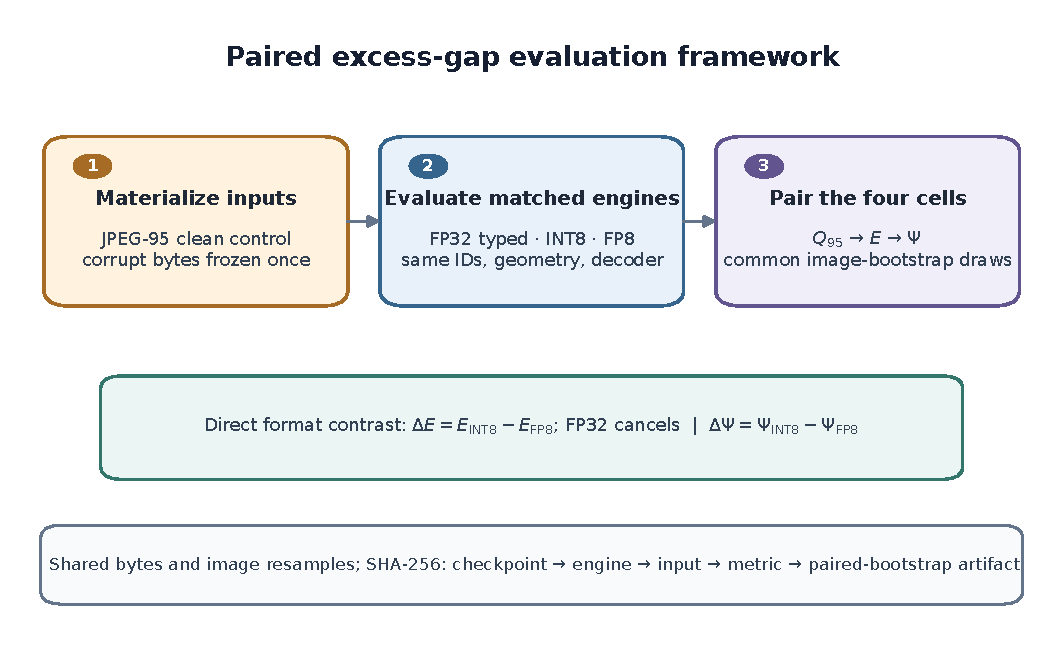
\includegraphics[width=\textwidth]{fig_framework.pdf}
\caption{Paired evaluation protocol. A deterministic JPEG-95 matched-clean
control and each corrupted input are materialized before the precision branch.
The direct four-cell block crosses INT8/FP8 with clean/corrupted input and is
resampled with common image draws. Matched-clean fidelity and absolute corrupted
AP are checked before the clean-adjusted interaction is interpreted.}
\label{fig:framework}
\end{figure*}

\subsection{Estimands and interpretation order}
\label{sec:estimands}

Let $d$, $m$, $q$, $b$, and $c$ index dataset, model, quantized treatment, size
endpoint, and corruption condition. The symbol $95$ denotes the matched clean
condition: no named corruption followed by deterministic JPEG quality 95 with
chroma subsampling disabled. All AP calculations use the native $[0,1]$ scale;
values are multiplied by 100 and reported as AP points.

The format-specific quantization gap is
\begin{equation}
Q_{d,m,q,b,c}=\AP_{d,m,\mathrm{FP32},b,c}-\AP_{d,m,q,b,c}.
\label{eq:q}
\end{equation}
The excess corruption gap is
\begin{equation}
E_{d,m,q,b,c}=Q_{d,m,q,b,c}-Q_{d,m,q,b,95}.
\label{eq:e}
\end{equation}
Positive $E$ means that corruption widens the FP32-to-quantized gap beyond its
matched-clean value; negative $E$ means that the gap contracts.

For the direct comparison, define the clean and corrupted FP8--INT8 gaps
\begin{equation}
G_{d,m,b,x}=\AP_{d,m,\mathrm{FP8},b,x}-
             \AP_{d,m,\mathrm{INT8},b,x},\quad x\in\{95,c\}.
\end{equation}
The primary interaction is
\begin{align}
\Delta E_{d,m,b,c}
&=E_{d,m,\mathrm{INT8},b,c}-E_{d,m,\mathrm{FP8},b,c}\nonumber\\
&=G_{d,m,b,c}-G_{d,m,b,95}.
\label{eq:delta-e}
\end{align}
The FP32-typed reference cancels algebraically. Positive $\Delta E$ means that
the FP8--INT8 AP gap is larger under corruption than on matched clean; negative
$\Delta E$ means that the gap contracts. Neither sign states whether the
corrupted accuracy is operationally useful.

The absolute corruption loss for precision treatment $p$ is
\begin{equation}
D_{d,m,p,b,c}=\AP_{d,m,p,b,95}-\AP_{d,m,p,b,c}.
\label{eq:d}
\end{equation}
We call the protocol \emph{floor-guarded}, rather than floor-corrected, because
$D$ and corrupted AP are interpretation checks; they do not transform or censor
$\Delta E$.

For COCO, VOC, and KITTI, the size interaction is
\begin{equation}
\Psi_{d,m,q,c}=E_{d,m,q,S,c}-E_{d,m,q,L,c},
\end{equation}
with direct contrast $\Delta\Psi=\Psi_{\mathrm{INT8}}-
\Psi_{\mathrm{FP8}}$. TT100K uses an analogous original-box-height contrast.
Area and height endpoints are reported as separate measurement families.

Table~\ref{tab:measurement-contract} states the required interpretation order.
An engine that fails the application's matched-clean accuracy requirement is
not rehabilitated by a favorable interaction sign. A signed interaction is then
read together with absolute corrupted AP; efficiency is considered only after
these accuracy checks.

\begin{table*}[t]
\centering
\caption{Measurement contract. All linked contrasts share the checkpoint,
ordered images, materialized bytes, decoder, and image-bootstrap draw.}
\label{tab:measurement-contract}
\small
\setlength{\tabcolsep}{4pt}
\begin{tabular}{Y{2.45cm}Y{2.7cm}Y{4.65cm}Y{4.35cm}}
\toprule
Question & Quantity & Isolated comparison & Interpretation boundary \\
\midrule
Matched-clean fidelity & $Q_{95}$ or $G_{95}$ & Accuracy cost before any named corruption & Does not establish corruption behavior. \\
Absolute corrupted accuracy & $\AP_c$ and $D$ & Retained task accuracy and clean-to-corrupted loss & Guards against common convergence near an AP floor. \\
Format-specific interaction & $E=Q_c-Q_{95}$ & Corruption-induced change in one quantized treatment's FP32 gap & Conditional on the recorded reference and treatment. \\
Direct format interaction & $\Delta E=G_c-G_{95}$ & Change in the INT8--FP8 discrepancy; FP32 cancels & Not an intrinsic format ranking; report with clean and absolute AP. \\
Size interaction & $\Delta\Psi$ & Difference between small-like and large-like format interactions & Area and height endpoint families remain separate. \\
Efficiency & engine size and latency & Runtime of the accepted executable treatment & Engine-only timing is not end-to-end deployment latency. \\
\bottomrule
\end{tabular}
\end{table*}

\subsection{Finite-grid target and evidence layers}
\label{sec:evidence-layers}

The exploratory landscape contains
$4$ datasets $\times3$ YOLO11 capacities $\times4$ corruptions $\times3$
severities $=144$ direct cells. Its balanced macro is the arithmetic mean over
this finite prespecified grid,
\begin{equation}
\overline{\Delta E}_{\mathrm{grid}}=
\frac{1}{144}\sum_{d,m,c}\Delta E_{d,m,c}.
\end{equation}
It is not a population-weighted effect for an unspecified deployment stream.
Image-count, object-count, leave-one-dataset, and leave-one-corruption summaries
are reported as alternative descriptive targets.

The evidence layers answer different validity questions (Table~\ref{tab:evidence-hierarchy}).
The four-dataset grid is exploratory because VOC2007 test and the recorded KITTI
validation partition participated in the checkpoint-selection workflow. A
separate VOC/KITTI rerun uses untouched final partitions and retrained
checkpoints; it is the strongest split-independent evidence for the stated
conditional contrast, but it covers only two datasets. Seed, corruption
realization, fixed-universe, and architecture studies are sensitivity analyses,
not replications of one universal parameter.

\begin{table*}[t]
\centering
\caption{Evidence hierarchy and permitted interpretation.}
\label{tab:evidence-hierarchy}
\small
\setlength{\tabcolsep}{3.6pt}
\begin{tabular}{Y{2.55cm}Y{4.15cm}Y{4.1cm}Y{3.7cm}}
\toprule
Layer & Scope & Uncertainty or dependency examined & Permitted claim \\
\midrule
Exploratory landscape & 144 YOLO11 cells; 2,000 paired image draws & Finite-image uncertainty and factorial heterogeneity & Conditional map and finite-grid macro \\
Untouched holdout & VOC and KITTI; six retrained checkpoints; 72 cells & Evaluation-after-selection reuse on two transfer datasets & Strongest split-independent conditional estimate \\
Training and calibration seeds & YOLO11m; three transfer datasets; severity 5 & Recorded $3\times3$ seed crossing & Bounded descriptive seed sensitivity \\
Corruption realizations & 36 base conditions; three frozen realizations & Stochastic materialization dependence & Bounded realization sensitivity \\
Fixed class universe & One TT100K stress cell; 10,000 weighted draws & Sparse category composition & One-cell endpoint sensitivity \\
Architecture portability & RT-DETR-L and RetinaNet; point estimates & Transfer of one frozen PTQ recipe & Failure-revealing stress evidence, not format superiority \\
\bottomrule
\end{tabular}
\end{table*}

\subsection{Datasets and size endpoints}
\label{sec:datasets}

Table~\ref{tab:datasets} summarizes COCO val2017\citep{lin2014coco}, PASCAL
VOC2007 test\citep{everingham2015voc}, the recorded KITTI validation split
\citep{geiger2012kitti}, and TT100K test\citep{zhu2016tt100k}. VOC and KITTI
annotations were immutably converted to COCO format. The reported values are
therefore COCO-style measurements on derived annotations, not official VOC or
KITTI challenge scores; VOC difficult-object and KITTI
\texttt{DontCare}/difficulty semantics are not reproduced as leaderboard
metrics.

TT100K contains 3,067 of the 3,071 referenced test images because four upstream
files were unavailable. Its class map declares 221 categories, of which 136
occur in the retained annotations. COCO, VOC, and KITTI use original-pixel area
strata: small $<32^2$, medium $[32^2,96^2)$, and large $\geq96^2$ pixels.
TT100K uses original bounding-box height: XS $[0,12)$, S $[12,24)$, M
$[24,48)$, L $[48,96)$, and XL $[96,\infty)$ pixels. Its small-like endpoint
combines XS+S and its large-like endpoint combines L+XL.

\begin{table*}[t]
\centering
\caption{Frozen evaluation datasets. Counts refer to the converted annotations
consumed by the evaluator.}
\label{tab:datasets}
\resizebox{\textwidth}{!}{\begin{tabular}{llrrrrp{5.2cm}}
\toprule
Dataset & Split & Images & Objects & Declared/observed classes & Input px & Size strata \\
\midrule
COCO & val2017 & 5000 & 36781 & 80/80 & 640 & area: $<32^2$ / $[32^2,96^2)$ / $\geq96^2$ \\
VOC & VOC2007 test & 4952 & 12032 & 20/20 & 640 & area: $<32^2$ / $[32^2,96^2)$ / $\geq96^2$ \\
KITTI & validation & 1496 & 8128 & 8/8 & 640 & area: $<32^2$ / $[32^2,96^2)$ / $\geq96^2$ \\
TT100K & test & 3067 & 8181 & 221/136 & 1280 & height: XS/S/M/L/XL \\
\bottomrule
\end{tabular}
}
\end{table*}

\subsection{Training, checkpoint selection, and holdout rerun}
\label{sec:training}

YOLO11n, YOLO11m, and YOLO11x provide three capacities within one architecture
family\citep{jocher2024yolo11}. VOC and KITTI use $640\times640$ input; TT100K
uses $1280\times1280$ to retain more sign detail. The exploratory transfer
checkpoints were trained for 100 epochs with seed 20260807, deterministic mode,
automatic optimizer and batch selection, automatic mixed precision, eight data
workers, and zero patience. The recorded augmentation used HSV amplitudes
0.015/0.7/0.4, translation 0.1, scale 0.5, horizontal-flip probability 0.5,
and mosaic probability 1.0, disabled for the final ten epochs. MixUp, CutMix,
copy-paste, rotation, shear, and perspective were zero. The trainer-selected
\texttt{best.pt} defines every precision rung for a dataset--capacity block.
COCO uses the corresponding official pretrained checkpoints without retraining.

The untouched rerun uses a prospectively frozen split registry (seed 20260818).
For VOC, train2007+train2012 provide 8,218 training images, val2007 provides
2,510 checkpoint-selection images, and val2012 provides 5,823 untouched final
images. For KITTI, 1,496 images remain the selection partition; a deterministic,
class-covered 1,197-image subset of the remaining records is reserved for final
evaluation and 4,788 images are used for training. Every observed class occurs
in each final partition. Calibration images are drawn only from the
corresponding training split, and the confidence threshold, NMS, decoder, and
calibration protocol are frozen before final evaluation.

\subsection{Executable precision treatments and calibration}
\label{sec:precision-treatments}

Engines were built with TensorRT 11.1.0.106 on an NVIDIA GeForce RTX 5090 using
a 4096-MiB builder workspace. The FP32-typed reference does not explicitly
disable TF32; ``FP32'' therefore names the implemented TensorRT reference and
not strict IEEE FP32 execution for every kernel. This limitation does not affect
the direct $\Delta E$, because the FP32 term cancels in Eq.~\eqref{eq:delta-e}.
FP16 is accepted only when its matched-clean AP differs from the FP32-typed
engine by at most 1.0 AP point.

Calibration manifests contain deterministic 512-image selections from the
training split and exclude evaluation images. The rebuilt COCO ladder uses a
common list for INT8 and FP8. Quantized ONNX graphs were produced with the
recorded ModelOpt \texttt{int8} and \texttt{fp8} modes and entropy calibration.
Inspection of all 24 YOLO quantized graphs verified INT8 zero-point tensors for
INT8 Q/DQ nodes and \texttt{FLOAT8E4M3FN} zero-point tensors for FP8 Q/DQ
nodes. Activation scales are per tensor, weight scales use axis 0 (per output
channel), and stored zero points are zero. Selected weights and activations are
quantized; Sigmoid and other operations outside Q/DQ regions remain at runtime-
selected precision. Supplementary Table~S4 reports graph-level coverage.

The recorded software environment used PyTorch 2.11.0+cu128, Ultralytics
8.4.95, ModelOpt 0.45.0 for the rebuilt COCO ladder, ONNX 1.21.0, NumPy 2.4.4,
Pillow 12.2.0, OpenCV 5.0.0, NVIDIA driver 610.43.02, and batch size one.
Older transfer registries omit some build-metadata fields, but their retained
ONNX graphs expose the verified datatype, scale-axis, and zero-point semantics.

\subsection{Synthetic corruptions and execution controls}
\label{sec:corruptions}

The suite contains four selected synthetic image corruptions. Gaussian noise
uses $\sigma/255\in\{8,20,40\}$; linear motion-blur kernels use
$\{5,13,23\}$ pixels; fog strength/radius pairs are $(0.18,6)$, $(0.38,12)$,
and $(0.62,20)$; and JPEG qualities are $\{70,40,15\}$. Severity labels 1, 3,
and 5 are ordinal within a corruption family and are not physically comparable
across families. In the exploratory grid, stochastic noise fields and blur
angles are independently realized across severity labels because severity is
part of the deterministic seed. Severity margins are therefore descriptions of
the recorded materializations, not within-image causal dose--response effects.

Every output is deterministically encoded as JPEG quality 95 with chroma
subsampling disabled, and dimensions are preserved. Each manifest records the
ordered image IDs, per-file hashes, dimensions, and generator parameters. The
matched-clean control applies the same materialization without a named
corruption. Corruptions are never generated inside an inference worker.
Letterbox geometry, inverse mapping, a confidence threshold of $10^{-3}$,
class-wise NMS at IoU 0.7, and a cap of 300 detections are held fixed. Run
records bind the engine, decoder, annotations, class map, input manifest, image
order, and prediction identity.

\subsection{AP evaluation and paired uncertainty}
\label{sec:uncertainty}

AP is evaluated across IoU thresholds 0.50:0.05:0.95. The image is the
resampling unit. For each dataset, a deterministic schedule of 2,000 image-index
draws is reused across every linked clean/corrupted and INT8/FP8 arm. Repeated
bootstrap positions are represented as repeated evaluator entries with unique
replicate-local identities, preserving image multiplicity and stable score
ordering. This common schedule retains the covariance that would be lost by
subtracting independently bootstrapped format summaries.

Two-sided percentile intervals quantify finite-evaluation-image uncertainty
conditional on the frozen checkpoints, engines, calibration lists, decoder,
corruption materialization, and evaluation split. They do not propagate
training-seed, calibration-sample, engine-build, dataset-selection, or
corruption-population uncertainty. Cell-wise interval signs are exploratory and
are not multiplicity-adjusted discoveries. The joint grid, area, and TT100K
height endpoints are calculated within common draws using frozen balanced
weights. Area and height endpoints are never pooled.

TT100K resamples can change the effective set of positive classes after
zero-positive categories are omitted from an AP average. A targeted sensitivity
for TT100K/YOLO11m/motion blur/severity 5 therefore uses 10,000 positive-weight
Bayesian image-bootstrap draws and a category--endpoint universe fixed to the
full 3,067-image annotation. This is a separate sensitivity estimand, not a
replacement for the ordinary image bootstrap.

\subsection{Sensitivity designs}
\label{sec:sensitivities}

\paragraph{Corruption realization.}
YOLO11m is evaluated on class-covering 512-image subsets of VOC, KITTI, and
TT100K with realization seeds 202608181, 202608182, and 202608183. Within an
image and realization seed, the stochastic field or angle is held fixed while
severity changes its magnitude; JPEG is deterministic. The design contains 36
base conditions and 108 realization cells. A nested summary resamples the three
realization labels and uses the paired image draw at the same replicate index.
With three fixed realizations, this is a bounded sensitivity analysis.

\paragraph{Training and calibration seeds.}
For YOLO11m on VOC, KITTI, and TT100K at severity 5, training seeds 20260807,
20260813, and 20260814 are crossed with three deterministic 512-image
calibration lists generated from the same seeds. Only the training and
calibration-list seeds vary. The $3\times3$ crossing produces 54 engines and
108 direct dataset--corruption cells. Marginal means and ranges are descriptive;
no population seed variance is inferred.

\paragraph{Weighting and omission.}
The same 144-cell ledger is summarized by equal-cell, image-count, and
object-count weights, and after omitting each dataset or corruption family in
turn. These analyses examine aggregation dependence without creating new
inference runs.

\subsection{Architecture portability stress cases}
\label{sec:crossfamily-methods}

RT-DETR-L, an end-to-end transformer detector\citep{carion2020detr,
zhao2024rtdetr}, and RetinaNet-R50-FPN-v2, an anchor-based dense detector
\citep{lin2017focal,torchvision2026retinanet}, are evaluated on VOC, KITTI, and
TT100K. Each family uses one deterministic 100-epoch transfer checkpoint per
dataset and the same frozen 512-image train-only calibration identity within a
dataset. The INT8 and FP8 construction recipes are transferred without
family-specific retuning. The question is whether the recorded recipe ports to
a different graph, not what an optimized family-specific recipe could achieve.

The extension contains 234 original-source-clean/corrupted metric cells and 18
separately materialized JPEG-95 matched-clean cells. The main sign convention
is reconstructed from the compact ledgers:
\begin{equation}
E=(\AP_{\mathrm{FP32},c}-\AP_{q,c})-
  (\AP_{\mathrm{FP32},95}-\AP_{q,95}).
\end{equation}
The direct contrast remains $\Delta E=E_{\mathrm{INT8}}-E_{\mathrm{FP8}}$.
Only point estimates are available, so ranges and means are descriptive. Engine
latency uses three 30-s \texttt{trtexec} repetitions after a 5-s warm-up and
excludes preprocessing, host transfer, decoding, and NMS.

\subsection{Artifact integrity and analysis boundary}
\label{sec:integrity}

The external analysis and artifact-generation pipeline validates expected
factorial grids, provenance links, and SHA-256 bindings before producing the
CSV, JSON, LaTeX, and figure assets consumed by this manuscript. LaTeX does not
independently verify hashes; it consumes those prevalidated outputs. The direct
audit binds the paired components, common draw caches, absolute-accuracy ledger,
and deployment records. A separate canonicalization script reconstructs all
144 cross-family interactions from the distributed corrupted and matched-clean
ledgers and asserts the sign convention before generating the manuscript table.
A second deterministic script derives the decision-impact figure and checks its
144-cell sign and AP-floor inventories. The source package includes these
manuscript-level scripts and their audits.

AI-assisted coding and language tools were used to refactor manuscript-level
validation scripts, check internal consistency, and revise the text. They did
not select experimental conditions, generate detector predictions, or replace
human interpretation. Every script operates on frozen ledgers, contains explicit
cardinality and sign assertions, and was reviewed and rerun by the authors; the
authors remain responsible for the analyses and claims.

\section{Results}
\label{sec:results}

\subsection{Execution integrity and matched-clean fidelity}
\label{sec:clean-results}

All 12 prespecified FP16 consistency gates passed the 1.0-AP-point tolerance.
The largest absolute FP32-typed--FP16 difference was 0.540 AP points
(TT100K/YOLO11x), and the largest among the COCO/VOC/KITTI area-evaluated
blocks was 0.253. These checks exclude gross disagreement within the recorded
TensorRT ladder; they do not estimate engine-build variance or prove exact
source-checkpoint parity.

On the JPEG-95 matched-clean inputs, FP8 achieved higher AP than INT8 in all 12
YOLO dataset--model blocks. The mean advantage was 1.40 AP points, ranging from
0.08 on TT100K/YOLO11x to 3.97 on KITTI/YOLO11m. This is the most consistent
format difference in the study: the recorded FP8 treatment preserves more clean
accuracy. It does not determine how the difference changes under corruption.

\subsection{Clean adjustment changes the practical interpretation}
\label{sec:decision-impact}

The raw corrupted FP8--INT8 gap was positive in 134 of 144 cells and averaged
1.38 AP points. Read alone, this result would suggest an almost uniform FP8
advantage under corruption. The matched-clean FP8--INT8 gap, however, was
positive in all 144 cells and averaged 1.40 points. After removing it, the mean
$\Delta E$ was -0.02 points; 78 cell estimates were positive and 66 were
negative. Most importantly, 56 cells had a positive raw corrupted gap but a
negative clean-adjusted interaction (Fig.~\ref{fig:decision-impact}A). No cell
changed in the opposite direction. The adjustment therefore changes the
scientific claim in 39\% of the grid, rather than merely rescaling the same
ranking.

Figure~\ref{fig:decision-impact}B links the signed interaction to the lower
corrupted AP of the two treatments. Eighteen cells place at least one format
below 10 AP and five place at least one below 5 AP. These cells illustrate why
clean adjustment and an absolute-AP guard answer complementary questions.

\begin{figure*}[t]
\centering
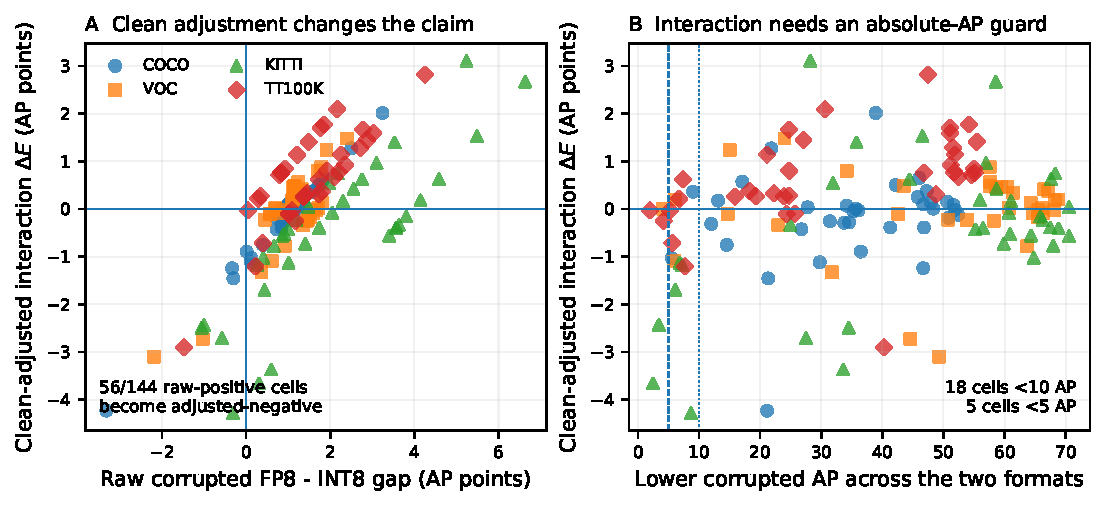
\includegraphics[width=\textwidth]{fig_decision_impact.pdf}
\caption{Decision impact of the protocol. (A) The raw corrupted FP8--INT8 gap
includes the matched-clean gap; 56 of 144 raw-positive cells become negative
interactions after clean adjustment. (B) The same interaction values are shown
against the lower corrupted AP across INT8 and FP8. Dashed and dotted vertical
lines mark 5 and 10 AP. Points are condition cells; colors and markers denote
datasets.}
\label{fig:decision-impact}
\end{figure*}

\subsection{Exploratory 144-cell interaction landscape}
\label{sec:exploratory-results}

Using common image-bootstrap draws, the balanced four-dataset
$\overline{\Delta E}_{\mathrm{grid}}$ was -0.02 AP points with a 95\%
percentile interval of $[-0.24,+0.15]$. The point estimates were highly
heterogeneous, ranging from -4.28 (KITTI/YOLO11m/motion blur/severity 5) to
+3.10 AP points (KITTI/YOLO11n/fog/severity 5). Dataset means also opposed one
another: TT100K was +0.61, whereas KITTI was -0.46 AP points
(Table~\ref{tab:dataset-margins}). Thus the near-zero macro is not evidence of
homogeneous zero interaction.

The separate area $\Delta\Psi$ over COCO, VOC, and KITTI was -0.50 AP points
with interval $[-1.18,+0.01]$. TT100K's height-based $\Delta\Psi$ was -1.38
points with interval $[-2.51,-0.14]$. Negative values mean that the INT8--FP8
interaction is more negative for the small-like endpoint than for the
large-like endpoint under the stated sign convention; they do not establish
that either format is robust on small objects. The full cell cloud and joint
endpoints are shown in Fig.~\ref{fig:paired-results}; the factorial sign
reversals are visible in Fig.~\ref{fig:heterogeneity}. Condition-level interval
counts and factor margins are reported in Supplementary Tables~S5--S6 and are
not treated as multiplicity-adjusted discoveries.

\begin{table}[t]
\centering
\caption{Dataset margins from the exploratory direct ledger. Values are AP
points; TT100K uses the height endpoint and the other datasets use area.}
\label{tab:dataset-margins}
\small
\resizebox{\columnwidth}{!}{% Compact dataset margins derived from generated/direct_format_contrast_cells.csv.
\begin{tabular}{llrrr}
\toprule
Dataset & Size endpoint & Cells & Mean $\Delta E$ & Mean $\Delta\Psi$ \\
\midrule
COCO & area & 36 & -0.19 & -0.12 \\
VOC & area & 36 & -0.04 & -0.44 \\
KITTI & area & 36 & -0.46 & -0.95 \\
TT100K & height & 36 & +0.61 & -1.38 \\
\bottomrule
\end{tabular}
}
\end{table}

\begin{figure*}[t]
\centering

\includegraphics[width=\textwidth]{fig_paired_excess_gap.pdf}
\caption{Exploratory direct interaction evidence. The left panel shows all 144
cell estimates and dataset means. The right panel shows joint paired-bootstrap
summaries for the finite four-dataset grid and the two non-pooled size endpoint
families.}
\label{fig:paired-results}
\end{figure*}

\begin{figure*}[t]
\centering
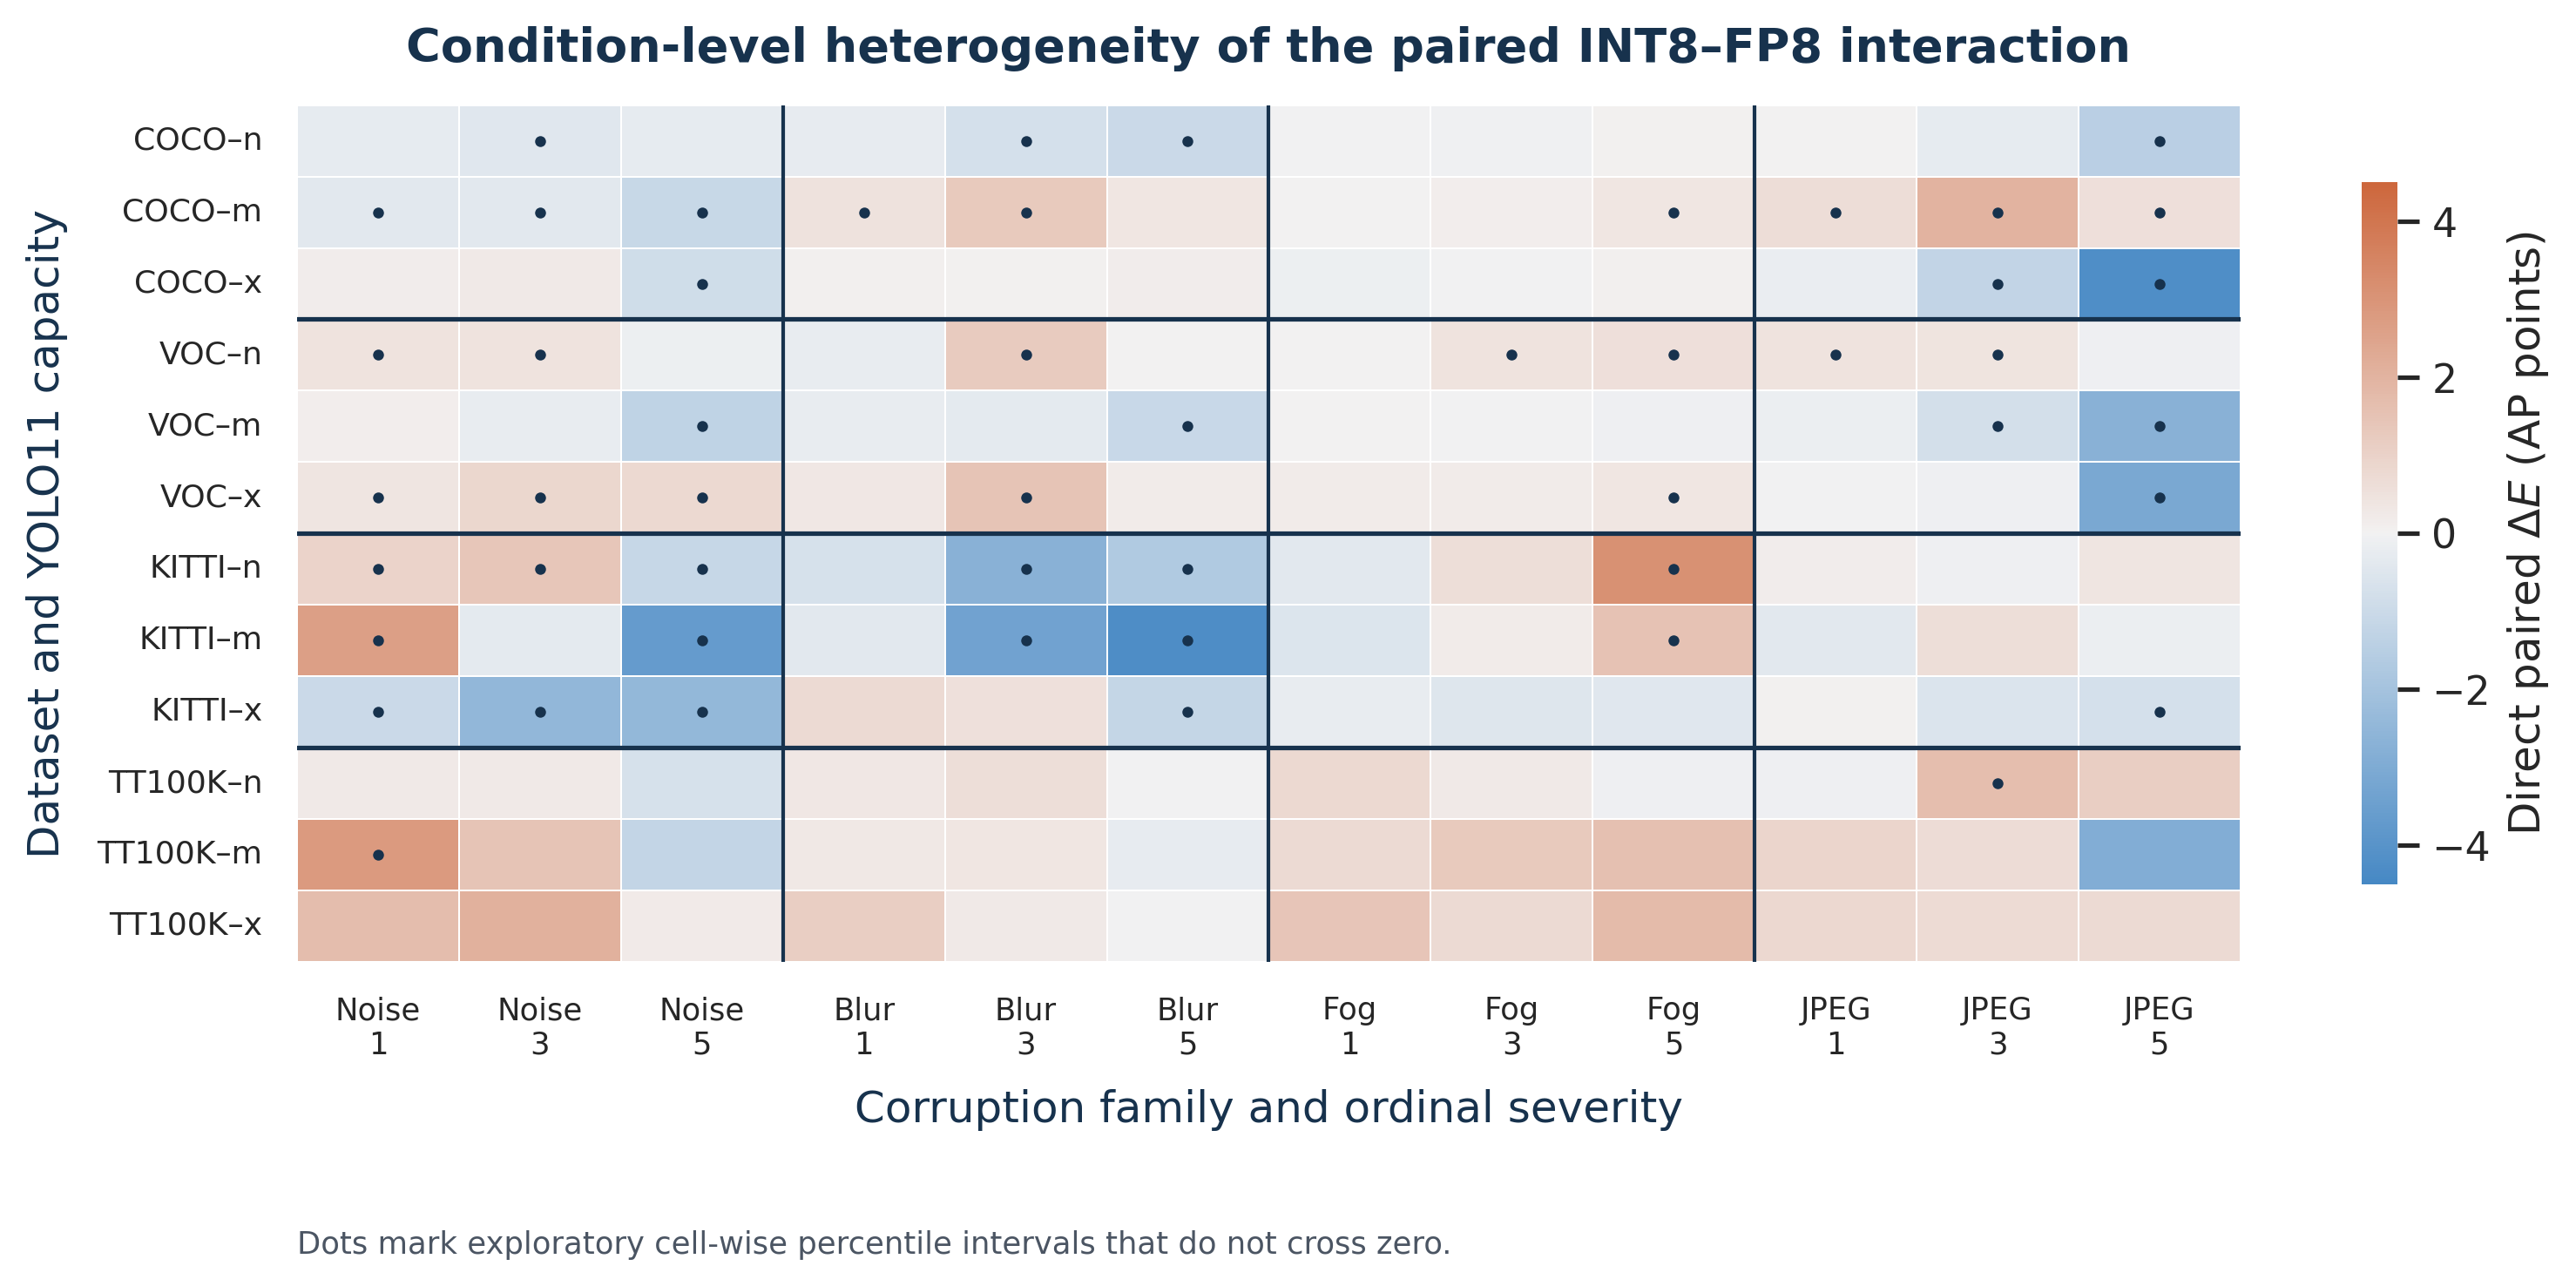
\includegraphics[width=\textwidth]{fig_direct_heterogeneity_heatmap.png}
\caption{Condition-level heterogeneity. Columns group corruption family and
ordinal severity; rows group dataset and YOLO11 capacity. Dots mark exploratory
cell-wise percentile intervals that do not cross zero; they are not
multiplicity-adjusted discoveries.}
\label{fig:heterogeneity}
\end{figure*}

\subsection{Untouched VOC/KITTI holdout evidence}
\label{sec:holdout-results}

The untouched rerun retains 72 equal-weight dataset--model--corruption--severity
cells. Its balanced direct interaction was -0.55 AP points
($[-0.78,-0.54,-0.29]$ for the 2.5th, 50th, and 97.5th percentiles). VOC was
-0.43 $[-0.54,-0.29]$ and KITTI was -0.67 $[-1.13,-0.20]$ (Table~\ref{tab:holdout}).
FP8 retained 1.60 more matched-clean AP on average and had a positive clean
advantage in all six dataset--model blocks. The size interaction was -0.13 AP
points with interval $[-0.98,-0.33,+0.38]$.

This rerun removes evaluation-after-selection reuse for these two datasets and
is therefore the strongest split-independent evidence in the paper. Its scope
is nevertheless narrower than the exploratory four-dataset landscape. The two
estimates answer different conditional questions and should not be pooled as
replications of one population parameter.

\begin{table}[t]
\centering
\caption{Untouched-holdout dataset margins. Effects and intervals are AP points
from the common paired schedule.}
\label{tab:holdout}
\small
\resizebox{\columnwidth}{!}{%
\begin{tabular}{lrrrrr}
\toprule
Dataset & Selection & Final & Cells & Mean $\Delta E$ & 95\% interval \\
\midrule
VOC & 2,510 & 5,823 & 36 & -0.43 & $[-0.54,-0.29]$ \\
KITTI & 1,496 & 1,197 & 36 & -0.67 & $[-1.13,-0.20]$ \\
\bottomrule
\end{tabular}}
\end{table}

\subsection{Absolute corrupted accuracy and floor guard}
\label{sec:absolute-results}

Across the 288 format-specific corrupted YOLO arms, 282 had lower AP than their
matched JPEG-95 clean arm. The median absolute loss was 5.51 AP points and the
mean was 15.24, revealing a strongly right-skewed degradation distribution.
Thirty-five arms fell below 10 AP and nine below 5 AP. In the untouched rerun,
18 of 144 corrupted format arms were below 10 AP and nine below 5 AP. These
counts show that a contracting format discrepancy can coexist with severe
absolute failure.

Table~\ref{tab:absolute-guardrail} reports balanced dataset--format summaries.
The all-corruption means hide substantial severity and condition variation, but
they make the interpretation boundary explicit: $\Delta E$ describes a change
in relative separation, not retained task performance. Size-specific absolute
AP and floor counts are provided in Supplementary Table~S2.

\begin{table*}[t]
\centering
\caption{Absolute-accuracy guardrail from the validated YOLO metric ledger.
$D=\AP_{95}-\AP_c$; rows are balanced descriptive summaries, not pooled
leaderboard scores.}
\label{tab:absolute-guardrail}
\small
\begin{tabular}{llrrrrr}
\toprule
Dataset & Format & Clean AP & All-corrupt AP & Mean $D$ & Severity-5 AP & Severity-5 $D$ \\
\midrule
COCO & INT8 & 46.010 & 34.911 & 11.099 & 25.185 & 20.826 \\
COCO & FP8 & 47.110 & 35.824 & 11.286 & 25.667 & 21.443 \\
VOC & INT8 & 65.732 & 49.246 & 16.486 & 35.478 & 30.255 \\
VOC & FP8 & 66.828 & 50.300 & 16.529 & 36.023 & 30.805 \\
KITTI & INT8 & 67.284 & 46.445 & 20.839 & 29.881 & 37.403 \\
KITTI & FP8 & 69.797 & 48.498 & 21.299 & 31.504 & 38.293 \\
TT100K & INT8 & 44.760 & 32.270 & 12.490 & 22.573 & 22.188 \\
TT100K & FP8 & 45.636 & 33.752 & 11.884 & 23.467 & 22.169 \\
\bottomrule
\end{tabular}

\end{table*}

\subsection{Sensitivity to weighting, realizations, seeds, and class universe}
\label{sec:sensitivity-results}

Alternative aggregation did not turn the small grid macro into a stable format
ranking. Equal-cell, image-count, and object-count means were -0.02, +0.00, and
-0.09 AP points, respectively, while the empirical cell SD was 1.20 points.
Leave-one-dataset-out means ranged from -0.23 to +0.13; leave-one-corruption-out
means ranged from -0.16 to +0.05. Sign changes around zero reflect conditional
heterogeneity rather than contradictory arithmetic.

The three-realization analysis over 36 base conditions produced a mean
$\Delta E$ of -0.23 AP points with nested percentiles
$[-0.95,-0.28,+0.37]$. Mean between-realization variance was 0.3989
AP-points$^2$, compared with mean within-image-bootstrap variance of 0.7446.
For $\Delta\Psi$, the mean was -1.04 with nested percentiles
$[-3.05,-1.42,+0.10]$. With only three materializations, these values bound a
recorded sensitivity rather than estimate a corruption population.

Across the targeted 108 training--calibration seed cells, the equally weighted
mean $\Delta E$ was -1.11 AP points. Training-seed marginal means ranged from
-1.64 to -0.68, and calibration-seed marginal means from -1.32 to -0.84. The
original-seed intersection was -1.21, close to the balanced seed-grid mean, but
the analysis covers only YOLO11m on three transfer datasets at severity 5.

For the fixed-universe TT100K stress cell, 10,000 positive-weight draws gave
$\Delta E$ percentiles $[-1.19,-0.17,+0.88]$, compared with
$[-1.79,-0.20,+1.34]$ under the ordinary 2,000-draw image bootstrap. The
median sign and zero-crossing status were unchanged. The height-based
$\Delta\Psi$ remained negative under both resampling schemes. Full sensitivity
tables are reported in Supplementary Sections~S7--S10.

\subsection{Engine-only runtime}
\label{sec:runtime-results}

Across the 12 matched YOLO dataset--model conditions, the median FP32-to-INT8
latency ratio was 2.96$\times$ (range 1.49--3.14$\times$), and the
FP32-to-FP8 ratio was 3.13$\times$ (1.78--3.36$\times$). The matched
INT8-to-FP8 ratio had a median of 1.08$\times$ and ranged from 0.92 to
1.19$\times$; FP8 was therefore not faster in every condition. Table~\ref{tab:runtime}
reports engine size, latency, and throughput. These measurements exclude image
decoding, preprocessing, transfer, detector decoding/NMS, power, and energy.

\begin{table*}[t]
\centering
\caption{RTX 5090 TensorRT engine measurements. Condition values are medians of
three raw-log-validated invocations; rows are medians across 12 matched
conditions.}
\label{tab:runtime}
\resizebox{0.82\textwidth}{!}{\begin{tabular}{lrrrr}
\toprule
Precision & Conditions & Median engine (MiB) & Median latency (ms) & Median throughput (qps) \\
\midrule
FP32 & 12 & 79.90 & 2.434 & 410.6 \\
INT8 & 12 & 24.07 & 0.789 & 1265.3 \\
FP8 & 12 & 21.92 & 0.760 & 1315.7 \\
\bottomrule
\end{tabular}
}
\end{table*}

\subsection{Architecture portability stress cases}
\label{sec:crossfamily-results}

FP8 remained within 1.15 matched-clean AP points of the FP32-typed engine in all
six RT-DETR/RetinaNet dataset--family blocks. The transferred INT8 recipe did
not preserve clean accuracy: its mean $Q_{95}$ was 38.66 AP points for RT-DETR-L
and 22.53 for RetinaNet. The largest failures were VOC/RT-DETR-L (69.30) and
KITTI/RetinaNet (43.30). Two FP32-typed transfer blocks were themselves weak:
RT-DETR-L/KITTI achieved 12.29 matched-clean AP and RetinaNet/TT100K 3.37.
These blocks are retained to expose transfer failure rather than excluded after
inspection.

Under the canonical $E=Q_c-Q_{95}$ sign, the mean INT8 interactions were -6.81
for RT-DETR-L and -6.21 AP points for RetinaNet. Mean corrupted INT8 AP was only
1.97 and 11.34, with 34/36 and 16/36 cells below 5 AP, respectively. FP8 mean
$E$ was near zero (-0.02 and +0.01) after much smaller clean gaps, with mean
corrupted AP of 33.30 and 26.91. The descriptive direct contrasts were -6.79
and -6.23 AP points. Figure~\ref{fig:crossfamily} shows why these negative
values are not evidence of INT8 robustness: they largely describe contraction
of a failed clean discrepancy near low absolute AP.

Both quantized treatments reduced engine-only latency relative to their family
FP32-typed reference. Median RT-DETR speedups were 2.47$\times$ for INT8 and
2.30$\times$ for FP8; RetinaNet speedups were 4.56$\times$ and 3.94$\times$.
The faster INT8 medians do not compensate for the clean-fidelity failure. The
supported conclusion is that the frozen recipe did not transfer, not that INT8
is intrinsically incompatible with either detector family.

\begin{figure*}[t]
\centering
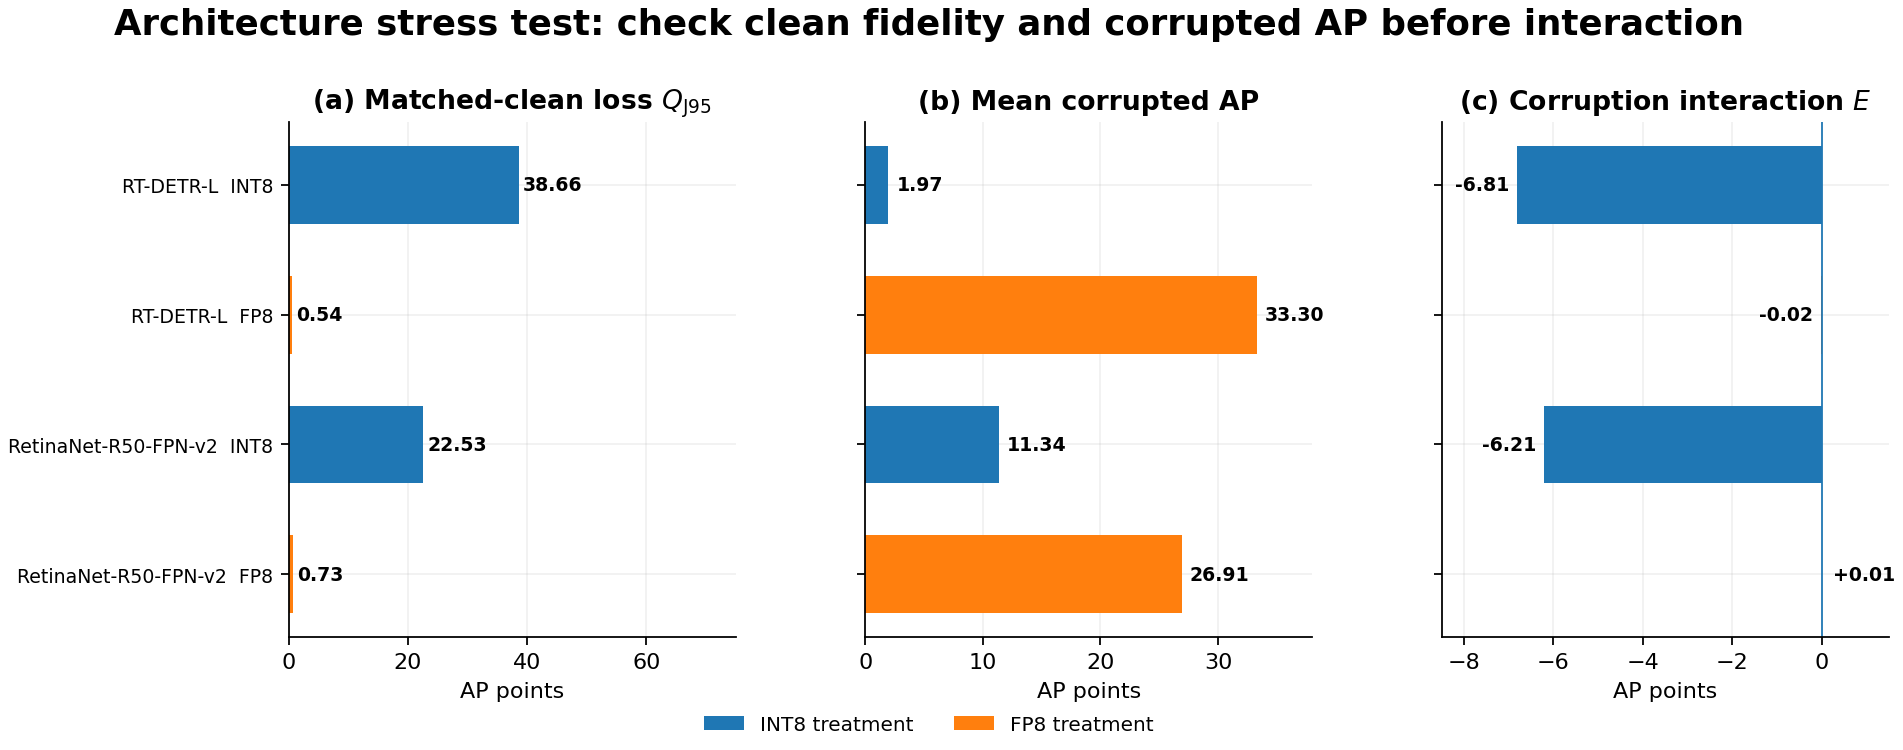
\includegraphics[width=\textwidth]{fig_cross_family_gates.png}
\caption{Architecture portability stress cases. Matched-clean loss is checked
first, interaction second, and absolute corrupted AP third. Each bar balances
VOC, KITTI, and TT100K. The negative INT8 interaction follows a large clean
accuracy failure and low corrupted AP.}
\label{fig:crossfamily}
\end{figure*}

\section{Discussion}
\label{sec:discussion}

\subsection{The protocol changes the question, not only the scale}

The clearest methodological result is the 56-cell interpretation change. A raw
corrupted FP8--INT8 gap favors FP8 in 134 of 144 cells, but the clean treatment
already favors FP8 in every cell. After that baseline discrepancy is removed,
66 interactions are negative and the balanced mean is near zero. The adjustment
therefore prevents a clean-fidelity result from being relabelled as a
corruption-robustness result. This distinction is consequential even when the
same engine, images, and AP evaluator are used: the choice of contrast changes
what can legitimately be concluded.

The direct formulation also improves statistical efficiency and clarity. The
four treatment arms remain inside each image draw, retaining the covariance
induced by common images, bytes, preprocessing, and decoder. Subtracting two
independently summarized format effects would discard that pairing and obscure
which uncertainty sources are shared. The algebraic cancellation of the
FP32-typed reference further isolates the treatment comparison from the TF32
status of that historical reference, while the format-specific $Q$ and $E$
decompositions remain available for diagnosis.

\subsection{Clean fidelity, absolute accuracy, and interaction are distinct}

FP8's 1.40-AP matched-clean advantage is consistent across all 12 YOLO blocks.
That result is stronger and more uniform than the corruption interaction. The
exploratory grid mean is -0.02 AP with an interval crossing zero, whereas the
untouched VOC/KITTI estimate is -0.55 with an interval below zero. A negative
$\Delta E$ means that the FP8--INT8 gap contracts relative to matched clean; it
does not mean that INT8 retains more useful corrupted accuracy or that FP8 is
fragile in an absolute sense.

The absolute guardrail is therefore not optional. AP falls in 282 of 288
corrupted YOLO arms, and 35 arms are below 10 AP. The architecture stress cases
make the same point more sharply: the transferred RT-DETR INT8 recipe begins
with a 38.66-AP mean clean gap, then shows a negative interaction while
retaining only 1.97 mean corrupted AP. The interaction sign is arithmetically
correct but operationally unhelpful without the preceding fidelity and floor
checks. For deployment, the evidence should be read in order: matched-clean
accuracy, absolute corrupted accuracy, interaction, and only then latency or
engine size.

The term \emph{floor-guarded} is intentionally modest. We do not propose a
formal correction for bounded AP or a thresholded primary estimand. Instead, we
make failure floors visible and prevent the signed contrast from carrying a
claim it cannot support. Applications can add predeclared minimum-AP or
maximum-loss gates appropriate to their risk tolerance; such gates should be
specified before the interaction is inspected.

\subsection{Why the exploratory and holdout estimates differ}

The four-dataset landscape and the untouched VOC/KITTI rerun have different
conditional scopes. The broader grid includes COCO and TT100K, three capacities,
and evaluation partitions that were not uniformly independent of checkpoint
selection. It maps heterogeneity across a finite factorial design. The holdout
rerun removes evaluation-after-selection reuse for VOC and KITTI and retrains
six checkpoints under frozen split registries. Its -0.55-AP estimate is the
strongest split-independent evidence available here, but it does not cover COCO,
TT100K, additional training seeds, or alternative detector families.

The difference between -0.02 and -0.55 should therefore not be treated as a
failed replication. It shows that the interaction depends on the target regime.
This interpretation is consistent with the exploratory dataset margins,
leave-one-factor summaries, and 1.20-AP cell dispersion. Reporting one pooled
number without its finite-grid definition would hide that dependence. A future
confirmatory study should predeclare the deployment-weighted target, construct
untouched partitions for every domain, and propagate training, calibration,
engine-build, and acquisition uncertainty in one hierarchical design.

\subsection{Heterogeneity and object size}

The near-zero grid mean is produced by opposing condition effects rather than a
uniform absence of interaction. Dataset margins range from -0.46 on KITTI to
+0.61 on TT100K, and cell estimates span more than seven AP points. Alternative
weights and leave-one-factor summaries remain small but cross zero. This pattern
supports treatment- and regime-specific reporting rather than a single format
robustness rank.

The size endpoints also resist a simple narrative. The area-based
$\Delta\Psi$ interval reaches zero, whereas the TT100K height endpoint is
negative. These quantities compare the format interaction between small-like
and large-like objects; they do not measure absolute small-object resilience.
Size-specific AP is often low, particularly for TT100K XS instances, so floor
contraction can be stronger for the small endpoint. In addition, area thresholds
and original-box-height thresholds define different scientific objects and must
not be pooled. The results therefore do not support a universal claim that
quantization-corruption interaction is amplified on small objects.

\subsection{Treatment-level interpretation of INT8 and FP8}

The graph audit shows that both nominal formats are mixed-precision treatments
with architecture-dependent Q/DQ coverage. Calibration, scale granularity,
operator exclusions, TensorRT tactic selection, output parameterization, and
decoder behavior all contribute to the executable system. This treatment-level
view explains why the same nominal INT8 recipe can preserve YOLO accuracy yet
collapse on RT-DETR or RetinaNet. The portability stress test is valuable
precisely because it exposes failure rather than because it supplies a fair
cross-family leaderboard.

The evidence does not localize the cross-family INT8 collapse to a specific
layer, quantizer, runtime stage, or decoder. Repair would require output-level
parity checks, layer-wise sensitivity, alternative calibration, mixed-precision
rescue, quantizer-search methods, or quantization-aware training. Conversely,
FP8's close clean tracking across the six stress blocks is encouraging but
remains conditional on one recipe, one hardware/software stack, one training
seed, and one calibration list per dataset. Neither result establishes an
intrinsic property of the number format.

\subsection{Practical reporting recommendations}

For an executable detector comparison under corruption, we recommend the
following minimum report. First, define a matched-clean materialization and
show the clean format gap. Second, materialize each corruption independently of
precision and share the exact bytes across treatments. Third, estimate the
clean-adjusted format interaction inside common image resamples. Fourth, report
absolute corrupted AP or clean-to-corrupted loss, with any application-specific
accuracy gate declared in advance. Fifth, retain condition-level or stratified
results so that a balanced mean cannot conceal reversals. Finally, state the
full executable treatment and separate engine-only timing from end-to-end
latency.

These recommendations extend beyond INT8 and FP8. The same four-cell structure
can compare quantizers, mixed-precision policies, compilers, calibration
strategies, or hardware runtimes whenever a pre-existing clean discrepancy may
be confused with a distribution-shift interaction.

\subsection{Limitations}

Several limitations bound the conclusions. The corruption suite contains four
selected synthetic transformations and does not represent the distribution of
natural weather, sensor, compression, or domain shifts. Severity is ordinal and,
in the exploratory grid, stochastic realizations are not nested across levels.
The three-realization analysis is too small to estimate a population of possible
fields or angles.

The exploratory macro is a finite-grid arithmetic mean, not a deployment-
weighted population effect. The broad grid remains conditional on one primary
training seed and recorded checkpoint-selection workflows; the untouched rerun
covers only VOC and KITTI. The targeted seed crossing fixes YOLO11m, three
transfer datasets, and severity 5, and does not estimate full training or
calibration variance. Engine builds were not repeated, and the bootstrap
intervals condition on the frozen executable artifacts.

VOC and KITTI are evaluated through converted COCO-style annotations rather
than official challenge protocols. TT100K's sparse class universe can vary
under ordinary image resampling; the fixed-universe check covers only one stress
cell. The area and height endpoint families are not interchangeable. The
FP32-typed TensorRT reference may use TF32, although this does not affect the
direct $\Delta E$ algebra.

Runtime is measured on one RTX 5090/TensorRT stack and excludes preprocessing,
transfer, decoding, NMS, memory, power, and energy. Graph-level Q/DQ counts do
not reveal TensorRT kernel precision or fallback execution. The cross-family
extension uses point estimates, one training seed, one calibration identity,
and fixed recipes that were not optimized per architecture. Finally, the
compact submission package reproduces manuscript-level summaries from frozen
ledgers but does not redistribute datasets, checkpoints, engines, or raw
prediction payloads.

\section{Conclusion}
\label{sec:conclusion}

A corrupted-image difference between quantized detectors is not, by itself, a
robustness comparison. It combines any pre-existing clean-fidelity gap with the
additional change induced by corruption. We introduced a byte-matched,
image-paired, floor-guarded protocol that separates these quantities through the
direct interaction
$\Delta E=(\mathrm{FP8}-\mathrm{INT8})_c-
(\mathrm{FP8}-\mathrm{INT8})_{95}$ and interprets it only alongside matched-clean
and absolute corrupted AP.

The distinction changes the evidence. Although the raw corrupted gap favored
FP8 in 134 of 144 YOLO cells, clean adjustment changed the interpretation in 56
cells. FP8 preserved 1.40 more matched-clean AP on average across all 12 YOLO
blocks, whereas the balanced exploratory interaction was -0.02 AP points with a
95\% interval of $[-0.24,+0.15]$. Untouched VOC/KITTI final partitions yielded
-0.55 $[-0.78,-0.29]$, demonstrating a narrower but stronger split-independent
conditional result. Absolute accuracy fell in 282 of 288 corrupted arms, with
35 below 10 AP, so gap contraction cannot be equated with retained performance.
Architecture stress cases further showed that a negative interaction can arise
when an INT8 recipe already fails its matched-clean fidelity gate.

The supported conclusion is not a universal INT8--FP8 robustness ranking.
Clean fidelity, absolute corrupted accuracy, and the corruption-specific format
interaction are different deployment claims. Reporting them together, under an
explicit finite target and a fully specified executable treatment, produces a
more auditable and decision-relevant evaluation of quantized computer-vision
systems.


\FloatBarrier
\section*{Data and code availability}

The source package and Supplementary Data~S2 supplied with this submission
contain the LaTeX source, generated CSV/JSON ledgers, validation audits, and
deterministic scripts needed to reproduce the manuscript-level summaries,
cross-family sign checks, and decision-impact figure. Raw benchmark datasets,
training checkpoints, TensorRT engines, and raw prediction payloads are not
redistributed because of licensing and size constraints. The retained run and
metric records bind the reported summaries to those artifacts by SHA-256. The
public source and compact evidence package is archived as software release
v2.0.0 at \url{https://doi.org/10.5281/zenodo.22031664}; the corresponding
repository is available at
\url{https://github.com/iamdinhthuan/paired-floor-guarded-int8-fp8-detection}.

\section*{Declaration of generative AI and AI-assisted technologies in the manuscript preparation process}

During manuscript preparation, the authors used OpenAI Codex, OpenAI ChatGPT,
and Anthropic Claude Code for language revision, LaTeX drafting, code
refactoring, and consistency checks. The tools did not autonomously select
experimental conditions or generate detector measurements. The authors reviewed
and reran the analysis and validation scripts, verified the numerical claims and
citations, edited the resulting text, and take full responsibility for the
content of the article.

\section*{Declaration of competing interest}

The authors declare that they have no known competing financial interests or
personal relationships that could have appeared to influence the work reported
in this paper.

\section*{CRediT authorship contribution statement}

\textbf{Dinh Thuan Nguyen:} Conceptualization, Methodology, Software,
Investigation, Formal analysis, Writing--original draft. \textbf{Lam Phuong
Nguyen:} Validation, Data curation, Writing--review and editing. \textbf{Vinh
Huy Nguyen:} Methodology, Visualization, Writing--review and editing.
\textbf{Mohan Rajesh Elara:} Supervision, Writing--review and editing.
\textbf{Anh Vu Le:} Supervision, Project administration, Writing--review and
editing.

\bibliographystyle{cas-model2-names}
\bibliography{references}

\end{document}
